%\documentclass[a4paper]{fhnwreport} %Legt grundlegende Formatierungen wie Schriftarten, Ort Seitenzahlen etc. fest.
%
%\graphicspath{{./graphics/}}%Change according to graphics folder!
%
%\begin{document}

\section{Hardware}

Der Hardware Teil ist in zwei Bereiche unterteilt: Sensorplatine und Kontrollplatine. Die Sensorplatine hat die Aufgabe die Spannungswerte der Solarzelle zu messen und diese über die Powerline an den Kontrollprint zu übermitteln.
Der Kontrollprint vergleicht diese Messwerte mit den Sollwerten einer funktionierenden Solarzelle und entscheidet dann ob dieses noch funtkionsfähig ist. Falls dem nicht so ist, wird eine Relaiskontakt geschlossen und ein Alarm mittels LED angezeigt. Auch wird auf einem Display angezeigt welches Panel defekt ist. 
Die Kommunikation zwischen diesen beiden Platinen darf keine zusätlichen Kabel benötigen, dies bedingt, dass die übermittelten Werte auf die Powerline moduliert werden müssen. Dieser Aufabu ist im Hardwarekonzept (Abbildung \ref{fig::Hardwarekonzept}) zu sehen.
%Der Sensorprint wird über das Solarpanel gespiesen. Es ist deshalb darauf zu achten, das die Leistung nicht mehr als 100mW beträgt.

%Die Kommunikation über die Powerline (PLC) wird mittels eines Powerline Transceivers/Receivers realisiert.
\begin{figure}[h]
\centering
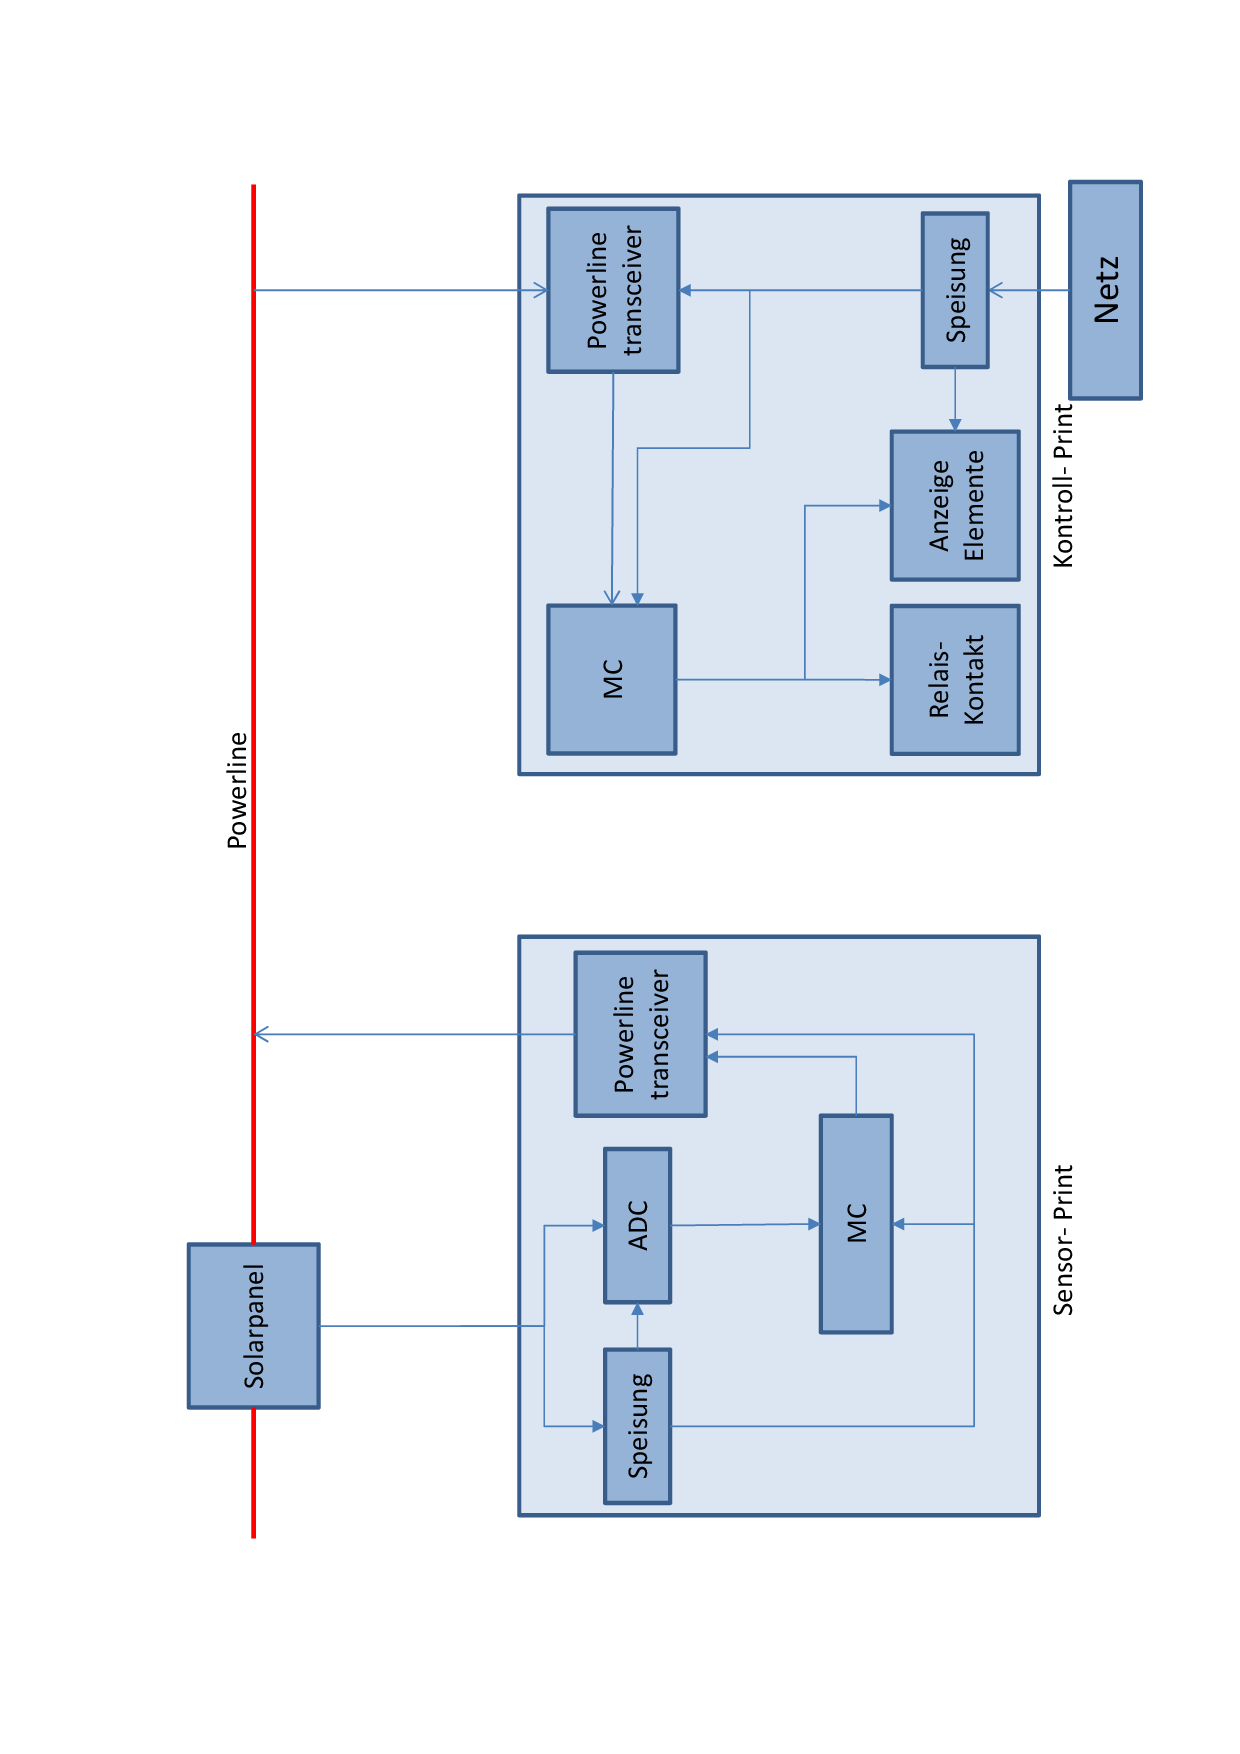
\includegraphics[angle = -90, width=1.0\textwidth]{Hardware_Konzept.png}%
\caption{Hardwarekonzept}
\label{fig::Hardwarekonzept}%
\end{figure}

\subsection{Sensorplatine}


Die Sensorplatine wird auf der Rückseite des Solarpanels angebracht. Es wird vom Solarpanel selbst gespiesen, weshalb auf möglichst kleine Leistungen geachtet werden muss. Die momentanen Spannungswerte des Solarpanels werden über einen AD-Wandler eingelesen und mit einem Microkontroller für den Powerline Transceiver entsprechend kodiert. Die kodierten Spannungswerte werden dann mittels eines Powerline Transceivers auf die Powerline eingekoppelt und so auf die Kontrollplatine übertragen.

\subsubsection{Powerline Transceiver}

Es wurde für einen Powerline Transceiver entschieden, da das Übertragungsprotokoll FSK (Frequency Shift Keying) schon gegeben ist und es aufgrund mangelnder Fachlichen Vorkenntnissen in einem zu grossen zeitlichen Aufwand resultieren würde, wenn diese Einkopplung in die Powerline selbst entwickelt werden würde. 
Dieser Transceiver hat die Aufgabe die vom Microkontroller kodierten Spannungswerte auf die Powerline zu übertragen.

\subsubsection{Spannungsmessung}

Die Spanungsmessung erfolgt über eine OP-Schaltung, welche de Spannungsbereich von 5-60V auf 0.42-5V hinabskaliert. Diese werden dann über einen AD-Wandler eingelesen und an den MC weitergegeben.

\subsubsection{AD Wandler}

Der AD Wandler soll mindestens 10 Bit Auflösung haben und die Werte seriell einlesen und ausgeben können. Dieser empfängt die skalierten Spannungswerte und digitalisiert diese für den Microkontroller.

\subsubsection{Microkontroller}

Der Microkontroller verschlüsselt die eingelesenen Werte nach FSK und sendet diese an den Powerline Transceiver.
\subsection{Kontrollplatine}

%\end{document}
